\documentclass{article}
\usepackage[utf8]{inputenc}
\usepackage{amsmath}
\usepackage{amssymb}
\usepackage{graphicx}
\usepackage[margin = 1 in]{geometry}



\title{CS5220: Matrix Multiply Project}
\author{Junyoung Lim, Max Ruth, Arjun Sharma}
\date{October 5, 2020}

\begin{document}

\maketitle

\section{Introduction}
As a group, we have tried a variety of ways to optimize matrix-matrix multiplication. We have found that improvements to our code have followed a couple of rules. 

First, copying large amounts is bad. For instance, as a form of copy optimization, we attempted to copy the whole of \texttt{A}, \texttt{B}, and \texttt{C} into structured aligned arrays. However, any potential improvement due to alignment was negated by the large amount of time moving memory. With more careful timing and storage, it is likely that alignment could be used to effect, but it would take much more attention to detail than simple copying. Another option would be to use the specific commands allowed by the Intel compiler, shown in the \texttt{kdgemm.c} example.

Second, large improvements in the flop rate could be made with simple changes to the code and compiler. For instance, after the addition of three compiler flags, changing the loop order of the basic code, and adding the \texttt{restrict} keyword, the speed of the code improved by approximately an order of magnitude, especially for small matrices. However, when we tried writing large amounts of code (e.g., when trying the copy optimization previously described), the performance tended to go down. 




References: 

https://stackoverflow.com/questions/38190006/matrix-multiplication-why-non-blocked-outperforms-blocked

https://suif.stanford.edu/papers/lam-asplos91.pdf


\section{Discussion: Compilation Details}
The simplest design decisions that we made were on the compiler side. We used the GCC 8.3.0 compiler that was downloaded by default in the \texttt{build-essential} package. The three flags that we used for the compilation are the following:
\begin{itemize}
	\item \texttt{-O3} --- Enable more aggressive optimization than the flag \texttt{-O2} used by default. 
	\item \texttt{-ffast-math} --- Allows the compiler to reorder operations that may not actually be associative. We did not see a dramatic increase in the error of the result using this flag, although there would be a chance for that when floating point operations are seen as associative. Perhaps for more pathological matrix examples, we might have to worry about this flag.
	\item \texttt{-march=native} --- Optimizes the code for the specific machine architecture. When running on a desktop with the flag \texttt{-fopt-info-vec}, adding \texttt{-march=native} changed the vectorization from 16 bytes to 32 bytes wherever possible - allowing a potential doubling of the computation speed.
\end{itemize}

Of course, there are likely many more compiler options that could have been considered. Our group did not experiment with the CLang, gfortran, or Intel compilers. From the 


\section{Discussion: the Inner Kernel}
The full code for our best inner kernel (found in \texttt{dgemm\_jki.c}) is given by:
\begin{verbatim}
void square_dgemm(const int M, 
                  const double* restrict A, const double* restrict B, double* restrict C)
{
    int i, j, k;
   
    for (j = 0; j < M; ++j) {			
        for (k = 0; k < M; ++k){
            for (i = 0; i < M; ++i) {
                C[j*M+i] += A[k*M+i] * B[j*M+k];
            }
        }
    }
}
\end{verbatim}

There are two major differences between this code and that of \texttt{dgemm\_basic.c}. First, this code has takes advantage of the \texttt{restrict} keyword when passing \texttt{A}, \texttt{B}, and \texttt{C}. This notifies the code that these matrices do not share pointers, and thus the output of \texttt{A[k*M+i] * B[j*M+k]} does not depend on the previous updates to the value of \texttt{C[j*M+i]}, allowing for GCC to vectorize the code appropriately. 

The difference between the loop with \texttt{restrict} and without is show in Fig.~\ref{fig:timing-jki-restrict}. We see that the Gflop rate of the \texttt{restrict} code is approximately twice that of the code for smaller matrices. This is because the computation in these situations is limited primarily by the processor and not by memory. For larger matrices, the primary limitation on computation speed moves to be memory, and the relative performances narrow, as neither is better than the other for memory hit rates.


\begin{figure}
    \centering
    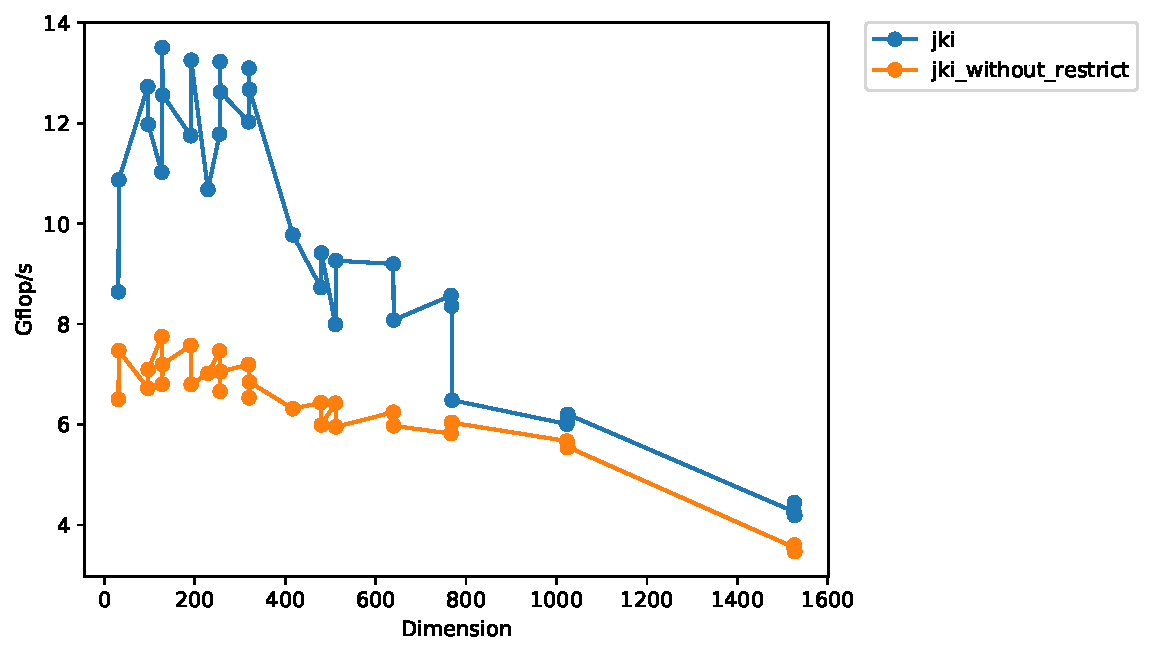
\includegraphics[width=0.6\columnwidth]{timing_jki_restrict.pdf}
    \caption{Flop rates for the inner \texttt{jki} kernel with and without the \texttt{restrict} keyword.}
    \label{fig:timing-jki-restrict}
\end{figure}

The second difference is the loop order. The \texttt{dgemm\_basic.c} code loops through the matrix multiplication in the \texttt{ijk} order, meaning the outside loop is in \texttt{i}, the middle is in \texttt{j}, and the inner is in \texttt{k}. However, this loop order is not particularly good for memory locality, as each iteration of the inner loop requires drawing upon an element of \texttt{A} that is \texttt{8M} bytes away. Note this is particularly important for the inner loop, as it is incremented a factor of \texttt{M} times more iterations than the middle loop and \texttt{M\^{}2} times more than the outer loop. Loading these elements quickly in succession is more difficult for this reason.

To address the locality issue, we choose the inner loop to be over \texttt{i}. This is because only the \texttt{i} iteration is local in all three matrices \texttt{A}, \texttt{B}, and \texttt{C}. The middle loop would then be over \texttt{k}, which has good locality in \texttt{B}, but not in \texttt{C}. Finally, the outer loop would be over \texttt{j}, which has the worst memory locality. 

We find that the numerical experiments shown in Fig.~\ref{fig:timing-loop-order} confirm this intuition. The two loop orders where \texttt{i} is the inner variable are faster than the rest, with the \texttt{jki} being the fastest of them all. 

\begin{figure}
    \centering
    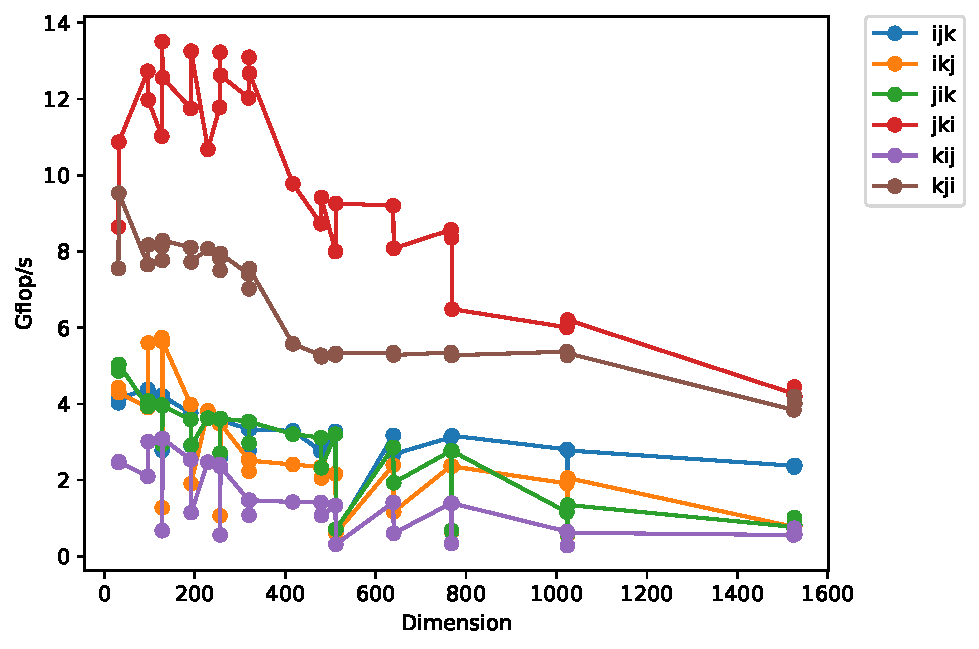
\includegraphics[width=0.6\columnwidth]{timing_loop_order.pdf}
    \caption{Flop rates for each of the six possible loop orders for the inner kernel.}
    \label{fig:timing-loop-order}
\end{figure}

We can learn a few other things from Fig.~\ref{fig:timing-loop-order}. For instance, it appears that when comparing between dimensions that are powers of two and their neighbors (such as the run 255, 256, and 257), the speed of the code can be significantly different. We believe this is likely related to associative caching. However, for small matrices that fit entirely into cache, it is unclear exactly why this would be an issue. We also see that these basic loop routines are strongest for small matrices, and tend to become significantly worse for large dimension. This could be interpreted via the roofline model, where smaller dimensions are bounded by flop rate (on the right side of the roofline) and the larger dimensions are bounded by memory efficiency (the left side of the roofline).




\section{Discussion: Blocking Strategies}
- Helps with associative cache
\subsection{Blocking}


%\section{Discussion: Memory management}

%\subsection{Copy Optimization}
% - free memory







\section{Conclusion}
\begin{itemize}
	\item We should have more carefully profiled our code. 
	\item Specific details about what is happening on a computer are important.
	\item BLAS is impressive, but weirdly slow for small matrices.
	\item Alignment is confusing
\end{itemize}



\end{document}